%%%%%%%%%%%%%%%%%%%%%%%%%%%%%%%%%%%%%%%%%
% Jacobs Landscape Poster
% LaTeX Template
% Version 1.0 (29/03/13)
%
% Created by:
% Computational Physics and Biophysics Group, Jacobs University
% https://teamwork.jacobs-university.de:8443/confluence/display/CoPandBiG/LaTeX+Poster
%
% Further modified by:
% Nathaniel Johnston (nathaniel@njohnston.ca)
%
% Modified further still by:
% Abraham Nunes (nunes <at> dal <dot> ca)
%
% License:
% CC BY-NC-SA 3.0 (http://creativecommons.org/licenses/by-nc-sa/3.0/)
%
%%%%%%%%%%%%%%%%%%%%%%%%%%%%%%%%%%%%%%%%%

%----------------------------------------------------------------------------------------
%	PACKAGES AND OTHER DOCUMENT CONFIGURATIONS
%----------------------------------------------------------------------------------------

\documentclass[final,table]{beamer}
\usepackage{multirow}

\usepackage[scale=1.24]{beamerposter} % Use the beamerposter package for laying out the poster
\usepackage{array}
\usetheme{confposter} % Use the confposter theme supplied with this template
\usepackage{bm}
\usepackage{xspace}
\usepackage{mathtools}
\usepackage{bm}
\usepackage{multirow}
\usepackage{adjustbox}
\setbeamercolor{block title}{fg=black,bg=} % Colors of the block titles
\setbeamercolor{block body}{fg=black,bg=} % Colors of the body of blocks
\setbeamercolor{block alerted title}{fg=white,bg=black} % Colors of the highlighted block titles
\setbeamercolor{block alerted body}{fg=black,bg=white} % Colors of the body of highlighted blocks
% Many more colors are available for use in beamerthemeconfposter.sty

\newcommand{\deemph}[1]{{\color{black!40}#1}}

%-----------------------------------------------------------
% Define the column widths and overall poster size
% To set effective sepwid, onecolwid and twocolwid values, first choose how many columns you want and how much separation you want between columns
% In this template, the separation width chosen is 0.024 of the paper width and a 4-column layout
% onecolwid should therefore be (1-(# of columns+1)*sepwid)/# of columns e.g. (1-(4+1)*0.024)/4 = 0.22
% Set twocolwid to be (2*onecolwid)+sepwid = 0.464
% Set threecolwid to be (3*onecolwid)+2*sepwid = 0.708

\newlength{\sepwid}
\newlength{\onecolwid}
\newlength{\twocolwid}
\newlength{\threecolwid}
\setlength{\paperwidth}{48in} % A0 width: 46.8in
\setlength{\paperheight}{36in} % A0 height: 33.1in
\setlength{\sepwid}{0.024\paperwidth} % Separation width (white space) between columns
\setlength{\onecolwid}{0.22\paperwidth} % Width of one column
\setlength{\twocolwid}{0.464\paperwidth} % Width of two columns
\setlength{\threecolwid}{0.708\paperwidth} % Width of three columns
\setlength{\topmargin}{-0.5in} % Reduce the top margin size

\makeatletter
\newcommand{\srcsize}{\@setfontsize{\srcsize}{5pt}{5pt}}
\makeatother

\setbeamerfont{bibliography entry author}{size=\tiny,}
\setbeamerfont{bibliography entry title}{size=\tiny}
\setbeamerfont{bibliography entry location}{size=\tiny,}
\setbeamerfont{bibliography entry note}{size=\tiny,}
%-----------------------------------------------------------

\usepackage{graphicx}  % Required for including images
\usepackage{amsmath} % assumes amsmath package installed
\usepackage{amssymb}  % assumes amsmath package installed
\usepackage[mathscr]{euscript}


% \usepackage{lmodern} % get rid of warnings
% \usepackage{caption} % improved spacing between figure and caption
%
% \DeclareCaptionLabelSeparator{horse}{:\quad} % change according to your needs
% \captionsetup{
%   labelsep = horse,
%   figureposition = bottom
% }
%
% \setbeamertemplate{caption}[numbered]
%
%
% % \setbeamerfont{caption}{size=\footnotesize}
% % \setbeamertemplate{caption}[numbered]
%


\usepackage{booktabs} % Top and bottom rules for tables
\usepackage{setspace}
\DeclarePairedDelimiter\abs{\lvert}{\rvert}%
\DeclarePairedDelimiter\norm{\lVert}{\rVert}%
\newcommand\Set[2]{\{\,#1\mid#2\,\}}

%----------------------------------------------------------------------------------------
%	TITLE SECTION
%----------------------------------------------------------------------------------------

\title{Plasticity and Evolvability in a Gene Regulatory Network Model} % Poster title

\author{Matthew Andres Moreno$^{1}$} % Author(s)

\institute{$^{1}$Michigan State University}% Institution(s)

%----------------------------------------------------------------------------------------

\setbeamerfont{caption}{size=\footnotesize}
\setbeamertemplate{caption}{%
    \structure{\textbf{\insertcaptionname~\insertcaptionnumber:}}
    \raggedright\insertcaption\par
}

\begin{document}
\addtobeamertemplate{block end}{}{\vspace*{1ex}} % White space under blocks1
\addtobeamertemplate{block alerted end}{}{\vspace*{0.5ex}} % White space under highlighted (alert) blocks

\setlength{\belowcaptionskip}{0ex} % White space under figures
\setlength\belowdisplayshortskip{2ex} % White space under equations

\begin{frame}[t] % The whole poster is enclosed in one beamer frame
\vspace{-1ex}
\begin{columns}[t] % The whole poster consists of three major columns, the second of which is split into two columns twice - the [t] option aligns each column's content to the top

\begin{column}{\sepwid}\end{column} % Empty spacer column

\begin{column}{\onecolwid} % The first column

%----------------------------------------------------------------------------------------
%	INTRODUCTION
%----------------------------------------------------------------------------------------
\begin{block}{Introduction}

\begin{alertblock}{Environment and Development}
\begin{figure}
 \centering
 
\includegraphics[width=\textwidth]{img/bioscheme}
 \caption{Genetic and environmental factors both influence the phenotype, which, in turn, determines fitness.}
 \label{fig:bioscheme}
\end{figure}
\end{alertblock}

\begin{alertblock}{Direct Plasticity
\cite{Fusco2010PhenotypicConcepts}}
\begin{figure}
\begin{columns}
\begin{column}{0.65\textwidth}
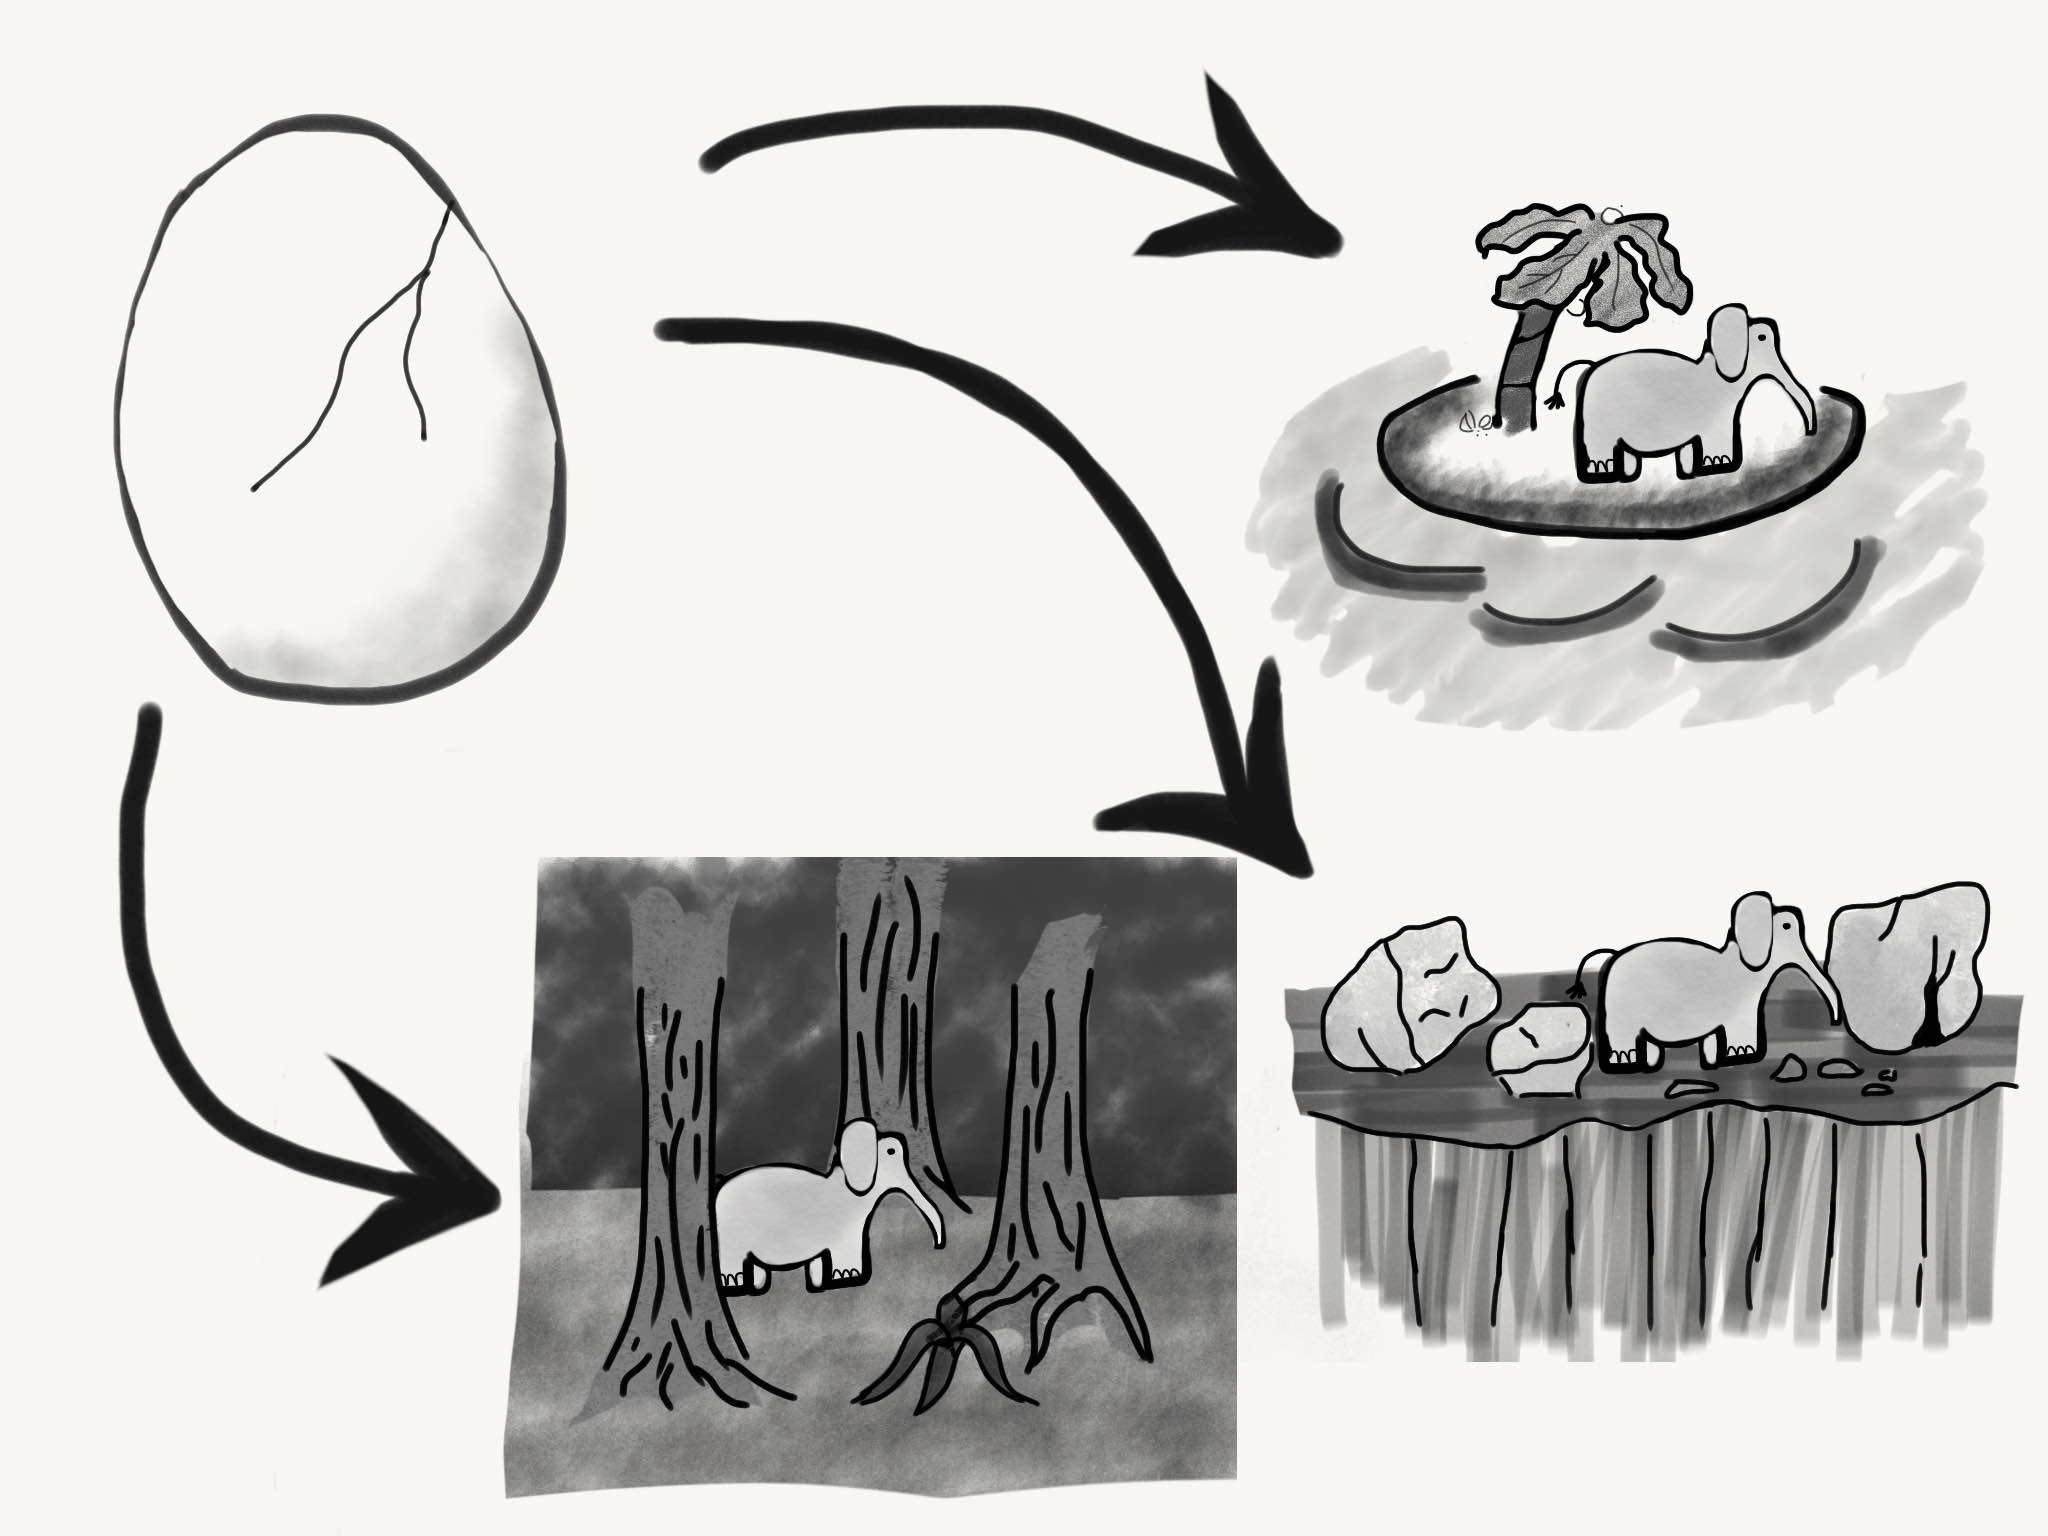
\includegraphics[width=\textwidth,trim={2cm 10cm 2cm 7cm},clip]{img/elephant_developmental_perturbation}
  %\captionsetup{singlelinecheck=off,justification=raggedright}
\end{column}
\begin{column}{0.3\textwidth}
  \caption{In this cartoon, phenotypic form is stable under environmental perturbation.}
  \end{column}
 \begin{column}{0.05\textwidth}
 \end{column}
 \end{columns}
  \label{fig:elephant_developmental_perturbation}
\end{figure}
\vspace{-2ex}
\end{alertblock}

\begin{alertblock}{Indirect Plasticity
\cite{Fusco2010PhenotypicConcepts}}
\begin{figure}
\begin{columns}
\begin{column}{0.65\textwidth}
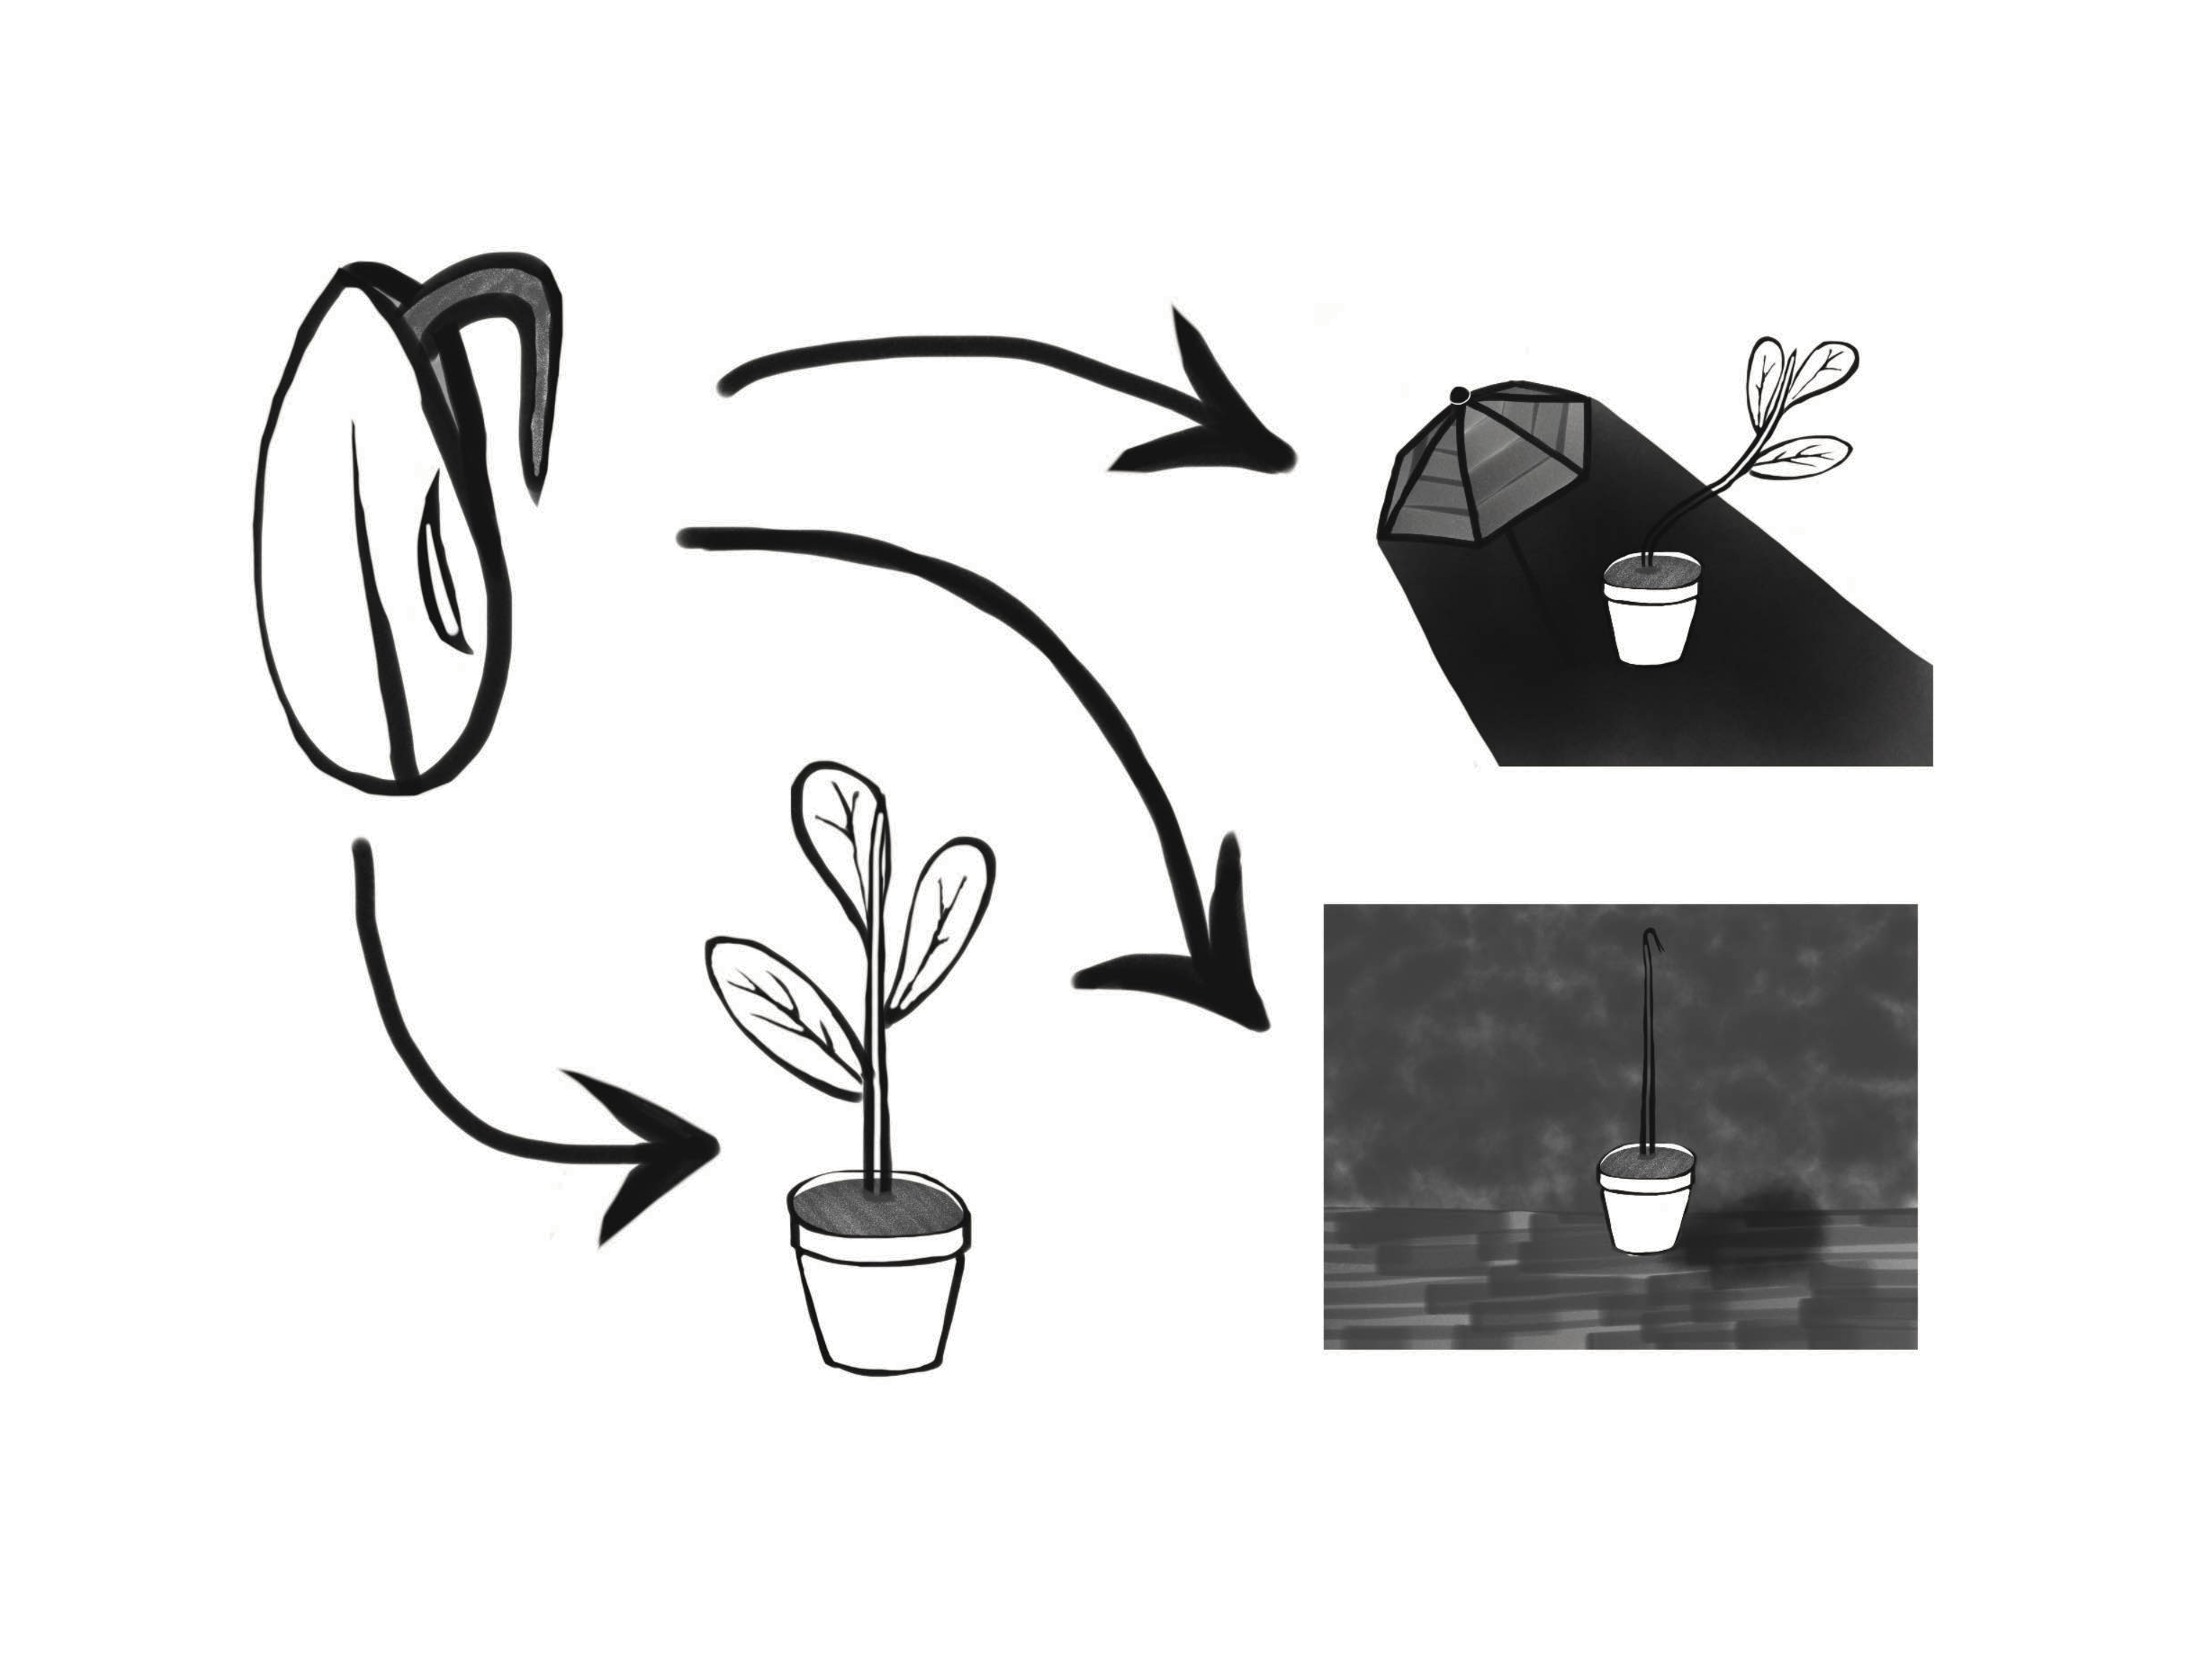
\includegraphics[width=\textwidth,trim={2cm 11cm 5cm 7cm},clip]{img/plant_developmental_perturbation}
  %\captionsetup{singlelinecheck=off,justification=raggedright}
\end{column}
\begin{column}{0.3\textwidth}
  \caption{In this cartoon, alternate phenotypes are expressed based on environmental signals.}
  \end{column}
  \begin{column}{0.05\textwidth}
  \end{column}
  \end{columns}
  \label{fig:plant_developmental_perturbation}
\end{figure}

\vspace{-2ex}
\end{alertblock}

\end{block}

\begin{block}{References}
{\tiny\bibliographystyle{abbrv}
\bibliography{bibl}}
\end{block}

\begin{block}{Acknowledgement}
{\footnotesize
Thank you Dr. America Chambers,	Dr. Adam Smith, Dr. Brad Richards, and Dr. Charles Ofria for your mentorship and feedback.
Thanks also to the authors of the Distributed Evolutionary Algorithms in Python and Scalable Concurrent Operations in Python packages.\par
}
\end{block}


%------------------------------------------------

%----------------------------------------------------------------------------------------
%	OBJECTIVES
%----------------------------------------------------------------------------------------


%----------------------------------------------------------------------------------------

\end{column} % End of the first column

\begin{column}{\sepwid}\end{column} % Empty spacer column

\begin{column}{\twocolwid} % Begin a column which is two columns wide (column 2)

%----------------------------------------------------------------------------------------
%	IMPORTANT RESULT
%----------------------------------------------------------------------------------------


\begin{block}{Model Components}
\vspace{-5ex}
\begin{tabular}{*{4}{>{\centering\arraybackslash}p{0.25\textwidth}}}
\begin{centering}

\includegraphics[width=0.20\textwidth]{img/placeholder}
\end{centering} &

\includegraphics[width=0.20\textwidth]{img/placeholder} &

\includegraphics[width=0.20\textwidth]{img/placeholder} & 

\includegraphics[width=0.20\textwidth]{img/placeholder} \\
\begin{spacing}{1.0}
\raggedright{\small
\textbf{Constant Power Propulsion} ants move fastest on slight decline}
\end{spacing} &
\begin{spacing}{1.0}
\raggedright{\small
\textbf{Food Attraction} magnitude increases exponentially with proximity to food}
\end{spacing} &
\begin{spacing}{1.0}
\raggedright{\small
\textbf{Nest Attraction} returner ant accelerates towards nest with constant magnitude}
\end{spacing} &
\begin{spacing}{1.0}
\raggedright{\small
\textbf{Near Nest Attraction} magnitude increases with nest proximity; acts $\perp$ to heading}
\end{spacing}
\\[-1.5cm]

\includegraphics[width=0.20\textwidth]{img/placeholder} &

\includegraphics[width=0.20\textwidth]{img/placeholder} &

\includegraphics[width=0.20\textwidth]{img/placeholder} &

\includegraphics[width=0.20\textwidth]{img/placeholder} \\
\begin{spacing}{1.0}
\raggedright{\small
\textbf{Role Switching} occurs 1cm from food (forager $\rightarrow$ returner) or nest (returner $\rightarrow$ forager)}
\end{spacing} &
\begin{spacing}{1.0}
\raggedright{\small
\textbf{Pheromone Deposit} rate proportional to ant speed (i.e. uniform per unit distance)}
\end{spacing} &
\begin{spacing}{1.0}
\raggedright{\small
\textbf{Pheromone Response} difference in pheromone between L and R determines magnitude}
\end{spacing} &
\begin{spacing}{1.0}
\raggedright{\small
\textbf{Pheromone Evaporation} rate proportional to pheromone concentration}
\end{spacing} \\[-1.5cm]

\includegraphics[width=0.20\textwidth]{img/placeholder} &

\includegraphics[width=0.20\textwidth]{img/placeholder} &

\includegraphics[width=0.20\textwidth]{img/placeholder} &

\includegraphics[width=0.20\textwidth]{img/placeholder} \\
\begin{spacing}{1.0}
\raggedright{\small
\textbf{``Boltzmann walker''} ant heading modified at occasional random reorientation events}
\end{spacing} &
\begin{spacing}{1.0}
\raggedright{\small
\textbf{Reorientation on Incline} random reorientation biased to alignments parallel to gradient}
\end{spacing} &
\begin{spacing}{1.0}
\raggedright{\small
\textbf{Arena Terrain} comprised of two flat sections joined by a simple incline}
\end{spacing} &
\begin{spacing}{1.0}
\raggedright{\small
\textbf{Nest/Food Placement} center-to-center shown in orange, corner-to-corner shown in purple}
\end{spacing} \\
\end{tabular}
\end{block}


\vspace{-1ex}

\vspace{1ex}
\begin{block}{Experimental Treatments}
\vspace{-1ex}
\begin{columns}
\begin{column}{0.5\textwidth}
\begin{alertblock}{Control}
\begin{figure}
    \centering
    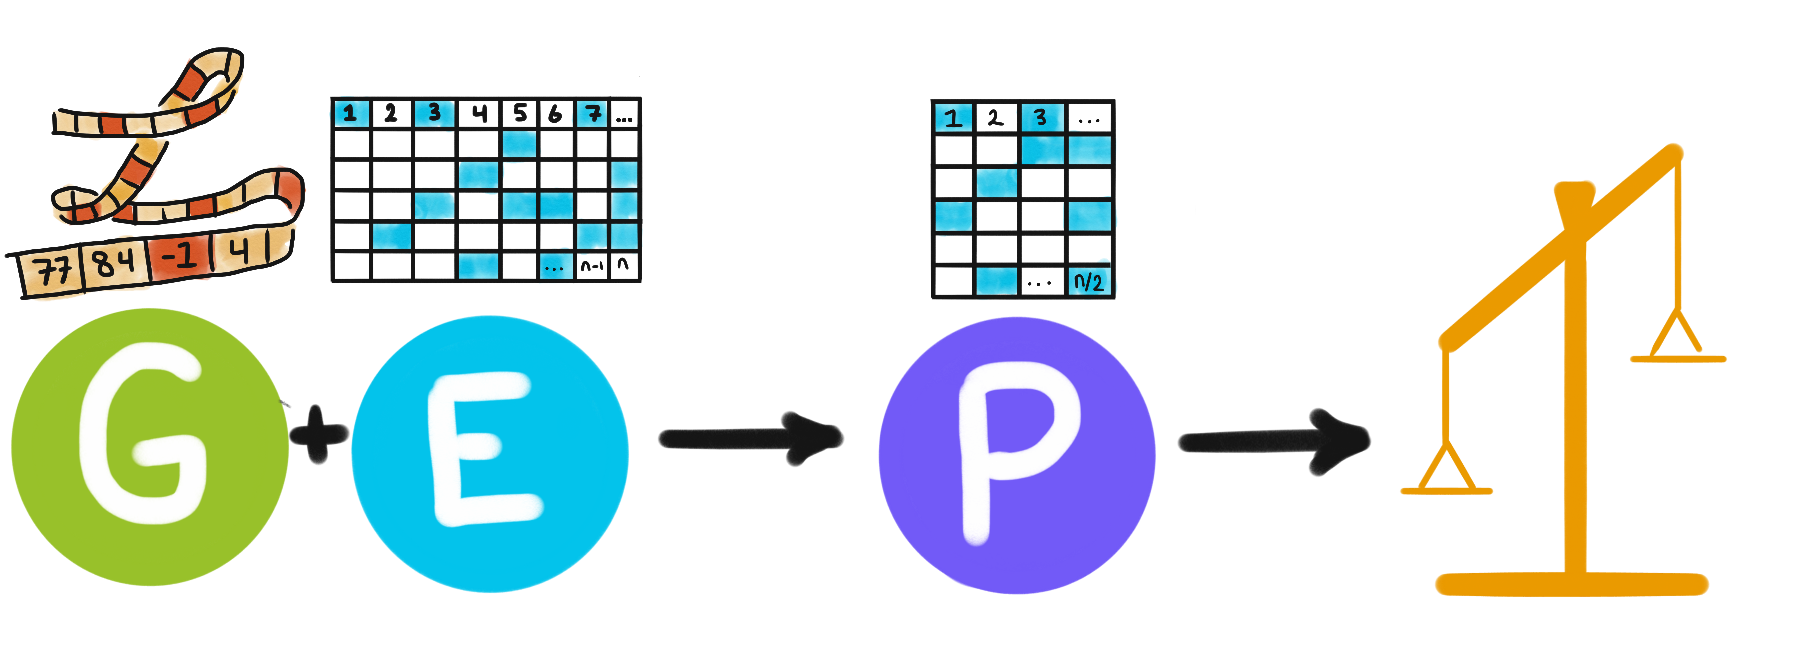
\includegraphics[width=0.8\textwidth]{img/modelscheme} \\
    \caption{In the control scheme, a static environment is used for each evaluation of a genotype.}
     \label{fig:control_scheme}
\end{figure}
\end{alertblock}
\begin{alertblock}{Direct Plasticity}
\begin{figure}
    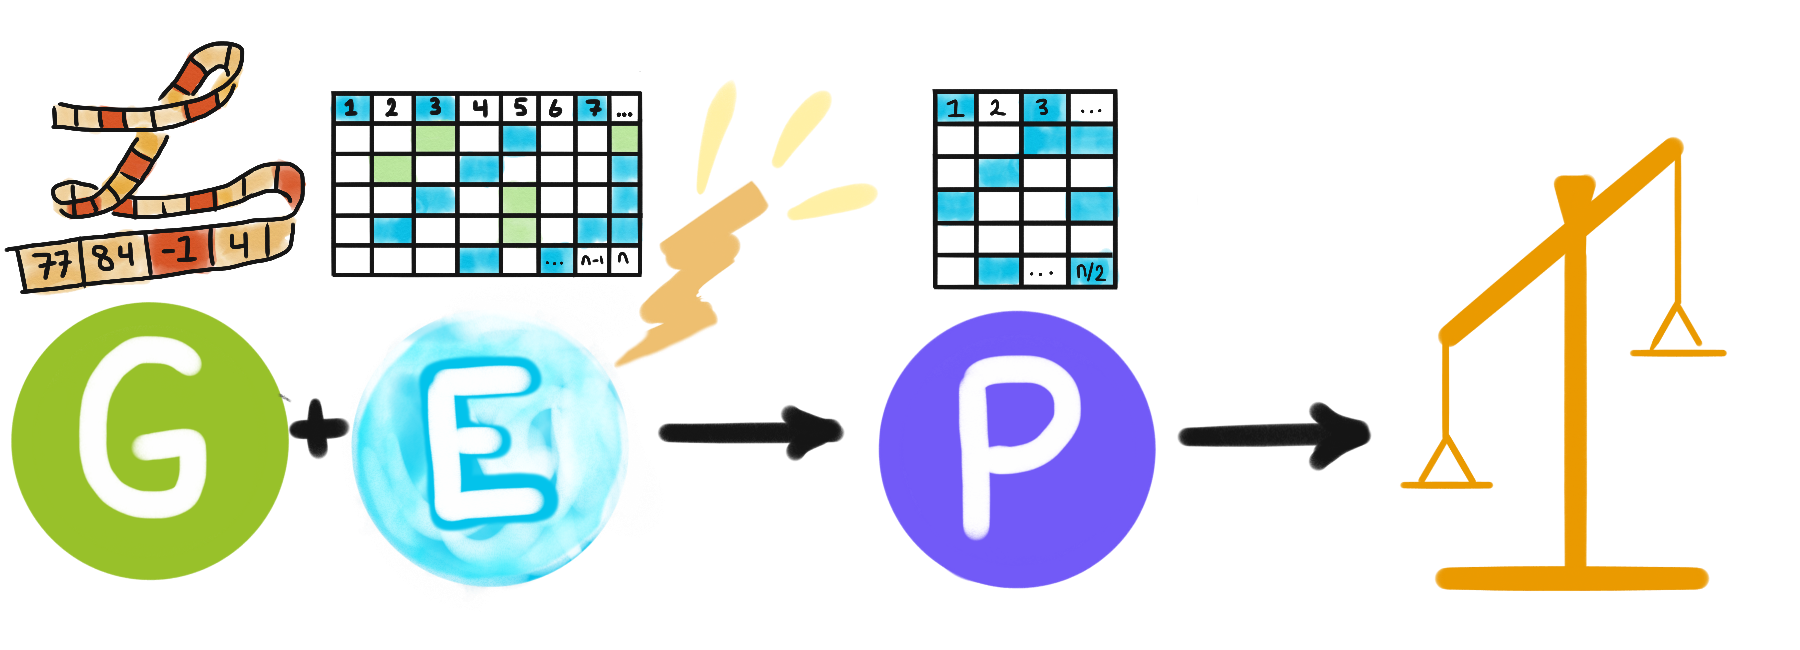
\includegraphics[width=0.8\textwidth]{img/directscheme}
  \caption{In the direct plasticity scheme, a subset of the initial environmental states are randomized for each evaluation of a genotype.}
  \label{fig:direct_plasticity_scheme}
\end{figure}
\end{alertblock}
\end{column}
\begin{column}{0.5\textwidth}
\begin{alertblock}{Indirect Plasticity}
\begin{figure}
    \centering
    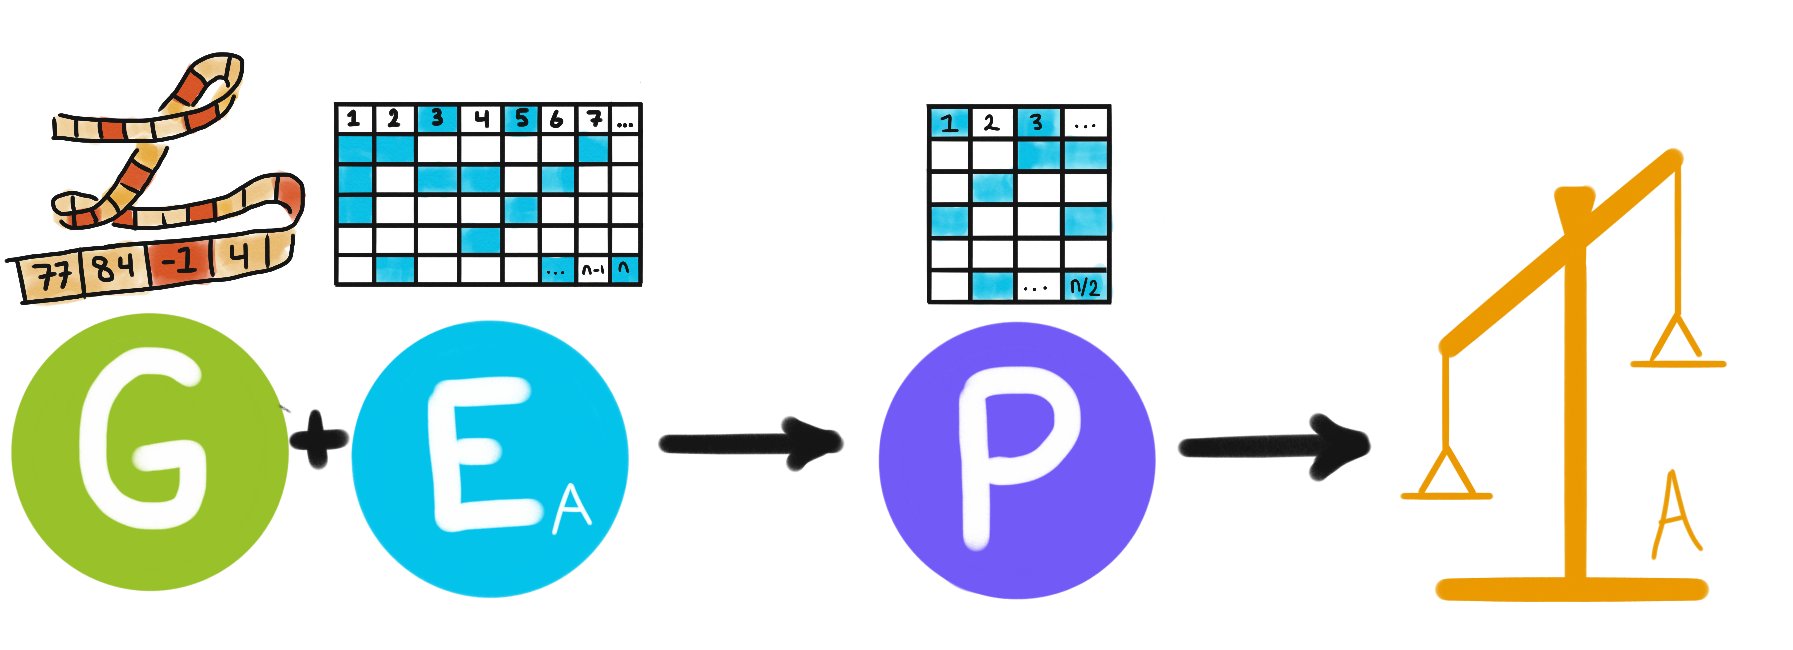
\includegraphics[width=0.8\textwidth]{img/indirectschemeA} \\
    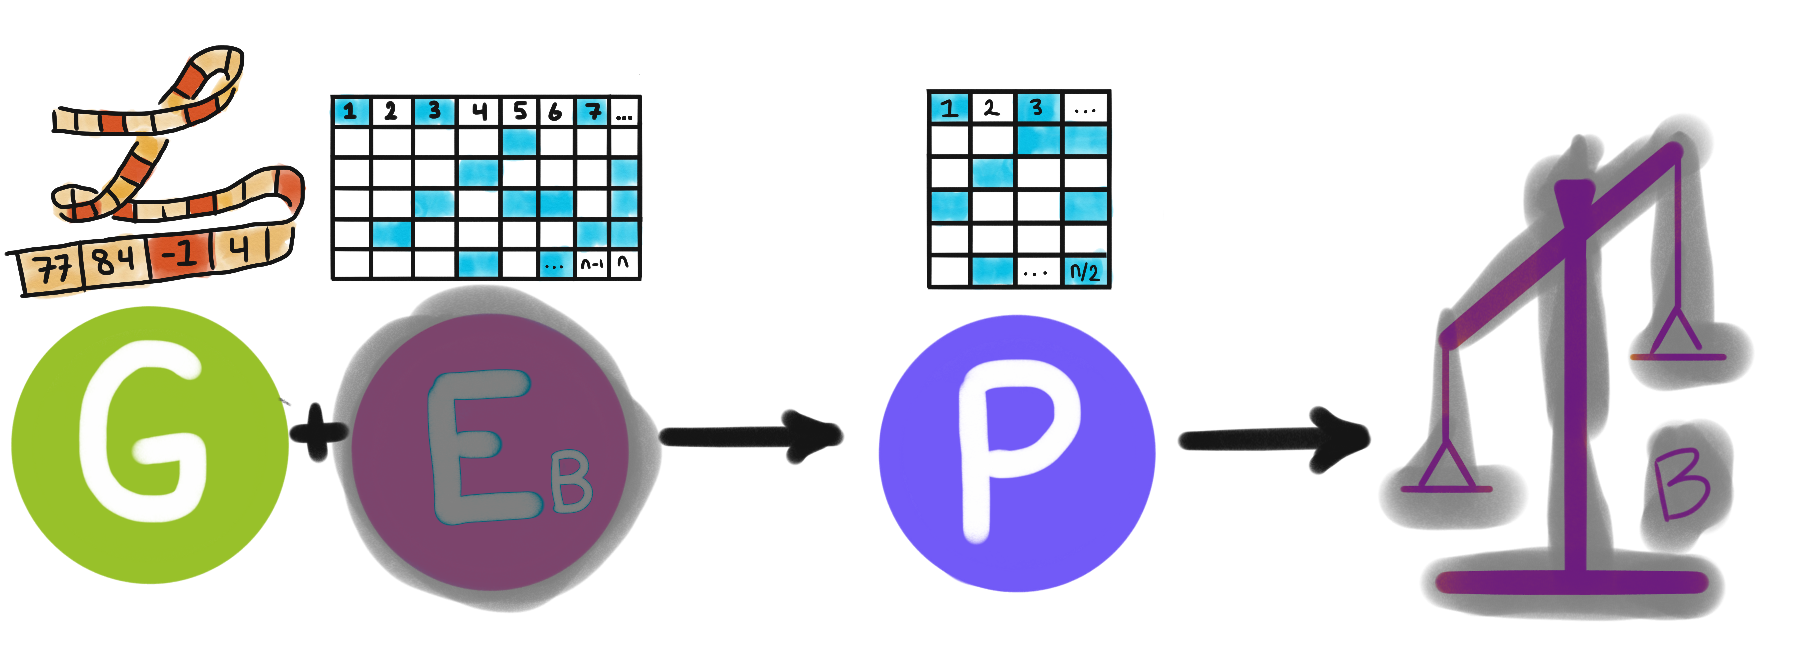
\includegraphics[width=0.8\textwidth]{img/indirectschemeB}
  \caption{In the indirect plasticity scheme, a pair of alternate environments signal which of two evaluation criteria is employed.}
  \label{fig:indirect_plasticity_scheme}
\end{figure}
\end{alertblock}
\end{column}
\end{columns}
\end{block}


%----------------------------------------------------------------------------------------
\vspace{-6ex}
\begin{columns}[t,totalwidth=\twocolwid] % Split up the two columns wide column again

\begin{column}{\onecolwid} % The first column within column 2 (column 2.1)


%----------------------------------------------------------------------------------------

\end{column} % End of column 2.1

\begin{column}{\onecolwid} % The second column within column 2 (column 2.2)


\end{column} % End of column 2.2

\end{columns} % End of the split of column 2

\end{column} % End of the second column

\begin{column}{\sepwid}\end{column} % Empty spacer column

\begin{column}{\onecolwid} % The third column

\begin{block}{Preliminary Results}
\begin{alertblock}{Direct Plasticity}
\begin{figure}
    \centering
    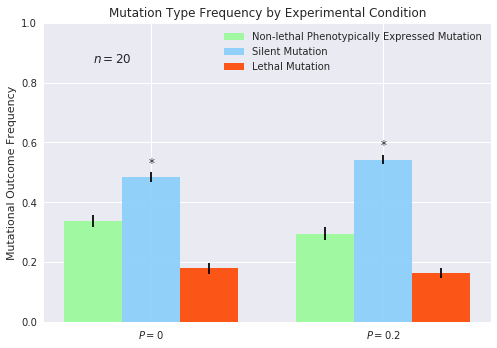
\includegraphics[width=\textwidth]{img/mutation_type_direct}
  	\caption{Champions evolved under a regime with initial state perturbation experience a higher rate of silent mutational outcomes.}
    \label{fig:mutation_type_direct}
\end{figure}
\end{alertblock}
\begin{alertblock}{Indirect Plasticity}
\begin{figure}
    \centering
    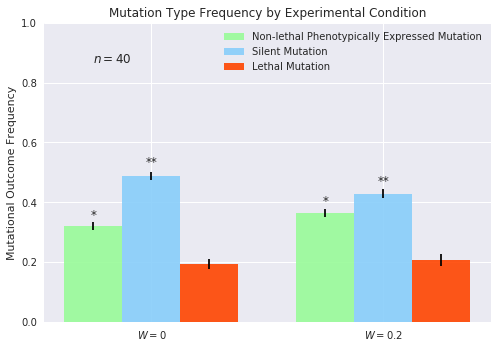
\includegraphics[width=\textwidth]{img/mutation_type_indirect}
  	\caption{Champions evolved with both primary and secondary condition/objective pairs experience a lower rate of silent mutational outcomes and a higher rate of nonlethal phenotypically observed mutational outcomes.}
    \label{fig:mutation_type_indirect}
\end{figure}
\end{alertblock}
\end{block}


\begin{block}{Next Steps}
\vspace{-1ex}
{\small
\begin{itemize}
\item investigate structural mechanism for observed differences in response to mutation 
\begin{itemize}
\item assess phenotypic outcomes of combined pairs of mutations  
\item assess skeletonized genotypes as graphs
\end{itemize}
\item investigate capacity of individuals evolved under different regimes to switch objectives
\item replicate results with more sophisticated model
\end{itemize}
}
\vspace{-1ex}
\end{block}



\end{column} % End of the third column

\end{columns} % End of all the columns in the poster

\end{frame} % End of the enclosing frame

\end{document}
